\documentclass{article}
\usepackage{icmc,amsmath}
\usepackage{graphicx}
\usepackage{url}
\usepackage[utf8x]{inputenc}
\usepackage[english]{babel}
\usepackage{color}

\title{Rameau: A System for Automatic Harmonic Analysis}

\oneauthor
  {Pedro Kröger, Alexandre Passos, Marcos Sampaio}
  {Genos---Computer Music Research Group\\ School of Music
   \\ Federal University of Bahia, Brazil \\
  \url{pedro.kroger@gmail.com}, \url{alexandre.tp@gmail.com}, \url{mdsmus@gmail.com}}

\newcounter{notacounter}

\newcommand{\nota}[1]{
  \addtocounter{notacounter}{1}
  \textcolor{red}{[nota \arabic{notacounter}: #1]}
}

\hyphenation{sim-ple-net}

\begin{document}
\maketitle

\begin{abstract}
%The abstract should be placed at the top left column and should contain
%about 150-200 words.

\end{abstract}

\section{Introduction}
\label{sec:introduction}

%% introducao geral

In music, harmonic analysis is the study of vertical sonorities and it
connections and is paramount to the understanding of tonal
compositions. The analyst can find the root of chords, label
sonorities with proper chords names (such as ``A minor''), and
identify the relationship between chords using roman numerals.

Harmonic analysis by computer is an important, challenging, and
interesting computer music research topic. It is challenging because
the musical material has a large variety of information such as
timber, notes, rhythm, dynamics, harmony, and by the fact that music is
not a linear process, unlike image \cite{mouton95:numeric}. The
harmonic changes in a choral texture, where usually all notes in all
voices begin and finish at the same time, are obvious. However, very
often chords can be arppeggiated, incomplete, and intertwined with
non-harmonic tones. These things contribute to increase considerably
the complexity for analysis \cite{pardo00:automated}. 

There are many practical applications for automatic music analysis,
among them arranging, detection of possible logical mistakes in
scores, database search, automatic accompaniment generation, and
statistical analysis of musical styles for automated composition
\cite{pardo02:algorithms,temperley99:modeling}. Computer-based
harmonic analysis is important because it can bring new insights in
music theory, in the same way the use of computer in vision and
problem solving has brought new insights in these areas
\cite{temperley99:modeling}.

Until now a single framework that allows the comparison between
different algorithms and analysis results has not been developed.
Pardo and Birmingham state that ``no researchers have published
statistical performance results on a system designed to analyze tonal
music'' \cite{pardo02:algorithms} before their paper. This lack of
data in literature makes it difficult to compare different systems.
Also, there aren't standard benchmarks to compare different algorithms
and analysis results. In fact, only Pardo and Birmingham
\cite{pardo00:automated} and Barthèlemy and Bonardi \nota{tinha o nome
  de Sleator aqui}
\cite{barthelemy01:figured} published specific comparisons between
different analysis results. Pardo and Birmingham compare their results
with Temperley and Sleator's \cite{temperley99:modeling} while
Barthèlemy compares his model against Maxwell's, Pardo and
Birmingham's, and Temperley and Sleator's
\cite{maxwell92:expert,temperley96:algorithm,pardo99:automated}.
However, these comparisons are based on results published in papers
and not from direct implementations. That means that only the examples
published by the authors can be compared.

In this paper we will present Rameau \nota{passos:achei melhor falar
  logo Rameau em vez de ``this system''}, a framework
\nota{passos:rameau é um framework, é bom deixar claro} for automatic
harmonic analysis of Western tonal music. Our main goal \nota{passos:
  o sistema não tem um objetivo, nós temos um em construí-lo} in
building this framework is to allow an easy comparison between
algorithms and results. \nota{falar limitacoes e escopo (harmonia
  tonal, corais de bach)} We also present an evaluation of ten
algorithms using a corpus of 150 Bach Chorales. Section
\ref{sec:system} describes Rameau in more details, section
\ref{sec:problem} lists the problems related to harmonic analysis,
section \ref{sec:analysis-results} analysis the results obtained, and
section \ref{sec:concl-future-work} .......

\section{The problem of automated harmonic analysis}
\label{sec:problem}

The problem of automated harmonic analysis might be understood by
dividing it into four sub-problems. 

The first problem is in the system's input format. If sharps and flats
are grouped together the program may have problems in places where
enharmonic information is important. Most systems either ignore this
problem or develop a pitch speller \cite{temperley99:modeling}. To our
knowledge no harmonic analysis software currently uses an input format
that preserves enharmonic information.

The second problem is determining what are the vertical sonorities in
a piece of music and grouping these sonorities into harmonically
significant segments, or chord-spans. This is called the segmentation
problem. Most of the difficulty of segmenting is due to the number of
possible segmentations of a piece being roughly an exponential
function of its length \cite{pardo02:algorithms}.

The third problem is labeling segments with chord names. Not every
segment forms a chord, though - some will consist solely of non-chord
tones and other melodic clues. Labeling a segment with a chord might
require contextual information, which complicates the matter a bit,
difficulting local decisions. Still, over 80\% of accuracy is possible
ignoring context (see section \ref{sec:analysis-results}).

The last problem is finding the key of the piece and assigning a tonal
function to each chord.

\section{The Rameau Framework}
\label{sec:system}

To properly study, understand and compare existing and proposed
algorithms for automated harmonic analysis we have designed and
implemented a framework , Rameau, that should enable us to

\begin{enumerate}
\item compare results precisely and repeatably with human analysis of
  a large corpus of music,
\item allow algorithms to access as much information as possible from
  the score used as input, and
\item easily develop new algorithms, test existing ones, and compare
  precisely the results.
\end{enumerate}

Reimplementing other algorithms in Rameau allows us to easily evaluate
their accuracy, study their errors and compare them with our baseline
techniques. We are unaware of research comparing many techniques for
harmonic analysis, in the manner of \cite{gomez.herrera:tonality}.

\subsection{Comprehensive Test Corpus}
\label{sec:comprehensive-test-corpus}

We are building a corpus of analyzed and digitalized Bach chorales to
use as training and test data. Bach chorales were chosen because:

\begin{enumerate}
\item they are easily analyzed (for example, the segmentation problem in
them consists simply of determining the sonorities), \nota{eles tem
  maior densidade de acorde por compasso que, por exemplo, uma sinfonia}
\item they are canonical examples of tonal harmony;
\item there are 371 on the Riemenschneider collection, more than
  enough for most needs; and
  \nota{porque isso é importante? passos: por serem muitos}
\item they have a simple structure, most with four voices forming
  simple triads and tetrads. \nota{explicar melhor, passos: bom, eu
    não seria a melhor pessoa para escrever essa parte, sinceramente,
    mas tentei fazer o meu melhor}
\end{enumerate}
\nota{passos:achei melhor enumerar como uma lista, assim quebra a repetição
  de analysis e padroniza melhor o parágrado}

We have already analyzed 150 of them and plan on completing this task
soon. The chorales are stored in a subset of the GNU Lilypond
\cite{nienhuys:lilypond} format, from which we generate MIDI files and
typeset scores, possibly annotated with analysis results (both by
human and by computer).

\subsection{Numeric codification for tonal music}
\label{sec:codificacao-jamary}

Probably the pitch-class notation, or some variation such as MIDI, is
the most used way of numerically representing pitch \nota{passos:
  troquei a ordem das palavras pra colocar pitch em ênfase, em vez de
  numeric}. The main problem with this notation is the loss of
enharmonic spelling \nota{passos: ``impossible to keep'' virou ``the
  loss''}. In this section we will revise three notations created
independently by Brinkman, Hewlett, and Oliveira
\cite{brinkman86:_binom_repres_of_pitch_for, hewlett92:base40,
  oliveira01:codificacao} to address this problem. For simplicity we
will refer to them as binomial, base-40, and base-96, respectively.

Notes in the binomial notation are represented as tuples in the form
of \texttt{<pc,nc>} where \texttt{pc} stands for pitch-class and
\texttt{nc} for note-class \nota{passos: achei bom especificar que são
  tuplas}. Note-class is a modulo 7 notation system that represents
numerically each note name (A, B, C, D, E, F, G) from 0 to 6. In this
system, for example C$\sharp$ is represented as \texttt{<1,0>} and
D$\flat$ as \texttt{<1,1>}. The binomial notation also allows a
compact \nota{passos: ``packaged'' fica confuso, uma tupla é mais
  ``packaged'' que um número, de certa forma, achei que ``compact''
  fica mais claro. kroger: brinkman usa packing e packaged}
representation using only one number per note \nota{passos: ``single
  numbers'' é confuso, é melhor usar ``one number per note'' ou
  simplesmente ``numbers''. brinkman (e outros) usa(m) single
  numbers}, where the pitch-class is multiplied by 10 and added to the
note-class. For example, C$\sharp$ becomes 10 and D$\flat$ 11.
\nota{<1,1> não seria D$\sharp$? nao é Db mesmo. passos: Certo. Então
  talvez seja melhor explicar melhor como se chega no resultado, eu
  mesmo só fui entender agora }

Unlike the binomial notation, the base-40 notation uses only single
numbers. The octave is divided linearly in 40 notes from C$\flat\flat$
to B$\sharp\sharp$. Table \ref{tab:base40} shows a few notes in this
system.

\begin{table}
  \centering
  \begin{tabular}{l|l}
    note & code \\
    \hline
    c$\flat\flat$ & 1 \\
    c$\flat$ & 2 \\
    c & 3 \\
    c$\sharp$ & 4 \\
    c$\sharp\sharp$ & 5 \\
    -- & 6 \\
  \end{tabular}
  \caption{A few notes in the base-40 notation}
  \label{tab:base40}
\end{table}

The base-96 notation is simple, elegant, and overcomes a few
shortcommings in both the binomial and base-40 notations. Since the
original publication of the base-96 notation is available only in
Portuguese, we will describe it here, comparing with the other
two.

The base-96 also is a numerical notation \nota{passos: ``single
  numbers'' sai daqui também.}. It has all the advantagens
of the base-40 notation with few advantagens. Table
\ref{tab:jama-notas} shows how notes are encoded. In this notation the
intervals are invariant under transformation \nota{passos:
  transposition fica mais claro que transformation (até onde eu sei é
  difícil algo ser invariante quanto a transformação). os intervalos
  podem ser os mesmos para diversas transformações (operações) com
  transposição, inversão, etc. passos: Então que tal ``invariant under
most transformations, such as...'' pra ficar mais claro?}. Table
\ref{tab:jama-intervalos} shows the coding for the intervals.

\begin{table}
  \centering
  \begin{tabular}{l|lllllll}
               & c & d& e& f& g& a& b \\
    \hline
    7$\flat$   &   & 7&21&  &  &62&76 \\
    6$\flat$   & 90& 8&22&35&49&63&77 \\
    5$\flat$   & 91& 9&23&36&50&64&78 \\
    4$\flat$   & 92&10&24&37&51&65&79 \\
    3$\flat$   & 93&11&25&38&52&66&80 \\
    2$\flat$   & 94&12&26&39&53&67&81 \\
    $\flat$    & 95&13&27&40&54&68&82 \\
    $\natural$ &  0&14&28&41&55&69&83 \\
    $\sharp$   &  1&15&29&42&56&70&84 \\
    2$\sharp$  &  2&16&30&43&57&71&85 \\
    3$\sharp$  &  3&17&31&44&58&72&86 \\
    4$\sharp$  &  4&18&32&45&59&73&87 \\
    5$\sharp$  &  5&19&33&46&60&74&88 \\
    6$\sharp$  &  6&20&34&47&61&75&89 \\
    7$\sharp$  &   &  &  &48&  &  &   \\
  \end{tabular}
  \caption{Notes in the base-96 notation}
  \label{tab:jama-notas}
\end{table}

\begin{table}
  \centering
  \begin{tabular}{l|llllllll}
    & 1$^{a}$& 2$^{a}$& 3$^{a}$& 4$^{a}$& 5$^{a}$& 6$^{a}$& 7$^{a}$& 8$^{a}$ \\
    \hline
    sd  &  & 7&21&35&49&62&76&90 \\
    pd  &  & 8&22&36&50&63&77&91 \\
    qd  &  & 9&23&37&51&64&77&92 \\
    td  &  &10&24&38&52&65&78&93 \\
    dd  &  &11&25&39&53&66&79&94 \\
    d   &  &12&26&40&54&67&80&95 \\
    m   &  &13&27&  &  &68&82&   \\
    J   & 0&  &  &41&55&  &  &96 \\
    M   &  &14&28&  &  &69&83&   \\
    A   & 1&15&29&42&56&70&84&   \\
    dA  & 2&16&30&43&57&71&85&   \\
    tA  & 3&17&31&44&58&72&86&   \\
    qA  & 4&18&32&45&59&73&87&   \\
    pA  & 5&19&33&46&60&74&88&   \\
    sA  & 6&20&34&47&61&75&89&   \\
    hA  &  &  &  &48&  &  &  &   
  \end{tabular}
  \caption{Invervals in base-96 notation}
  \label{tab:jama-intervalos}
\end{table}

The base-96 notation works for up to seven flats and sharps, witch is
more than enough for tonal music. This system is compatible with the
pitch-class system (modulo 12): in the base-96 notation G = 55, and
the result of 55 mod 12 is 7, representing G in the pitch-class
notation. \nota{passos: a parte do exemplo estava confusa, é melhor
  explicar menos e mostrar só como funciona, eu acho}

The base-40 notation starts to fail with notes that have more than two
accidentals. For example, the interval between C$\flat\flat$ and
C$\sharp\sharp$ (a quadruple augmented unison) has the same value (6)
as diminished second. On the other hand, in the base-96 notation this
interval can be correctly computed.

The main problem with the binomial notation is that operations that
are (and should be) simple become complex. In both base-40 and base-96
notations, transposition is as simple the adding \nota{passos: ``as
  simple as the sum'' não faz sentido, usando ``as simple as adding}
an index to a note, while in the binomial system it has to use two
different operations (mod and div) besides the addition. Its compact
\nota{passos: packaged -> compact} 
representation is supposed to simplify things, but as an example,
transposition become something like:

\begin{verbatim}
10 ((a div 10 + B div 10) mod 12)
 + ((a mod 10 + B div 10) mod 7)
\end{verbatim}

To do anything non-trivial, like interval-class vectors, yet extra
work has to be done, increasing complexity.

For these reasons we have adopted the base-96 codification, although
no algorithm at present makes direct use of it. We believe it is a
very nice form of describing tonal music numerically and it should be
more known among researches and developers.

\subsection{Answer sheet format}
\label{sec:formato-dos-acordes}

The results of human analysis performed on the chorales are stored in
a simple, flexible text format, designed to

\begin{enumerate}
\item be as close as possible to usual popular notation,
\item represent inherent ambiguities in chords (it is possible to name
  more than one chord as a possible analysis for a given sonority),
  and
\item single out sonorities that do not constitute chords, instead
  having melodic functions on the piece.
\end{enumerate}

The first four sonorities of the answer sheet for Bach's ``Aus meines
Herzens Grunde'' chorale (the first in our corpus), for example, are
stored as \texttt{G G C/E (C7+/E [b])}. Each chord symbols represents
a sonority. Chords in parenthesis represent possible interpretations
of a single sonority. Notes in brackets are non-chord tones, marking
sonorities that do not constitute chords.

This information is then used as anwer sheets and training data on the
many algorithms implemented in our system.

\subsection{Architecture}
\label{sec:architecture-and-api}

The architecture of the Rameau framework is simple. First, a score is
parsed (our parser is written using Cl-Yacc
\cite{chroboczek:_cl_yacc_manual} and Cl-Lexer
\cite{parker:_lexer_packag}) into a list of notes, which is then split
into a list of sonorities. Then, these sonorities are sent to each
algorithm for analysis. The analysis results and their comparison with
the answer sheets are then output either textually or as an annotated
score, as in figures \ref{fig:coral-12} and \ref{fig:coral-54}.

The algorithms used for analysis are implemented using a very simple
Common Lisp API. To implement one it is enough to place a lisp file in
a special directory and call the \texttt{register-algorithm} function
inside that file, specifying as parameter the algorithm's name, an
analysis function and a comparison function. The input to the analysis
function is a list of sonorities, which are lists of notes, each note
specifying its onset time, duration, octave and pitch. The output is a
list of either chords or non-chord tones, each chord possibly having a
fundamental, a mode, a seventh, a bass, and additions. The framework
provides a few possible comparison functions for easy usage.

We have currently implemented using this API 
\begin{enumerate}
\item a subset of the algorithm described in \cite{pardo02:algorithms}
  (ignoring, for now, segmentation), 
\item a port (work-in-progress) of the algorithm described in
  \cite{temperley99:modeling}, 
\item some neural networks (using the Fann \cite{nissen:fann}
  library) roughly similiar to some described in
  \cite{tsui02:_harmon_analy_using_neural_networ}, and
\item decision trees modeled after the neural networks (using code
  from \cite{Mitchell:1997:ML}).
\end{enumerate}

The code is publicly available, under a GNU GPL \cite{fsf:gpl} license
in a git \cite{baudis:_git_users_manual} repository at
\url{genos.mus.br/repos/rameau.git} and for visualization at
\url{git.genos.mus.br/?p=rameau.git}

\subsection{Comparison with similar software}
\label{sec:differences-from-similar-software}

We only had access to one similar system, Temperley and Sleator's
Melisma \cite{temperley99:modeling}. We had some issues parsing its
output, and so have been unable to reproduce their claimed
accuracy. We have a work-in-progress reimplementation of their
algorithm, averaging 60\% accuracy on the chorales it can handle.

Even though we couldn't find a public repository for Pardo and
Birmingham's HarmAn \cite{pardo99:automated}, from their article the
system seems to face most issues we found with the Melisma system. Our
re-implementation of their algorithm is based solely on the article.

Rameau differs from these systems mainly by our focus on testing the
results of many algorithms. Also common to most other systems is the
notion that in a musical piece every sonority is part of a chord (or
at least has a root). This is not true of sonorities containing
non-chord tones such as suspensions, passing notes and some voice
leading clues. It is one of our goals to get results as close as
possible to usual human analysis, so we classify these sonorities as
non-chord tones and any labeling of them with chords is seen as an
error.

\section{Preliminary results}
\label{sec:analysis-results}

\nota{é bom ter uma introdução. por exemplo: porque seções para NN e
  arvores e não para pardo? passos: por que eu não tinha nada para
  dizer sobre pardo, então coloquei algo}

As Rameau is a work-in-progress, most of our main questions regarding
automated harmonic analysis are still unanswered. We, however, already
have some insights on how the implemented techniques work, how do
their common errors look like and how some of them may be improved.

\subsection{Pardo and Birmingham's Algorithm}
\label{sec:pardo-birmingham}

The algorithm described in \cite{pardo99:automated} has some
interesting properties. It handles most simple examples of tonal
harmony really well, but has no clear notion, by design, of non-chord
tones, augmented chords and other possible analysis. We
have found no need, as of yet, of implementing the segmentation
algorithm, since segmentation is trivial in Bach Chorales.

The current accuracy is $66 \pm 9\%$.


\subsection{Neural Networks}
\label{sec:neural-nets}

Neural networks are a tool to perform non-linear statistical data
modeling that works by having artificial ``neurons'' exchange
information \cite{russell02:aima}. There are
many varieties of neural networks, each being more useful for a
certain type of problem. Our networks are all multilayer feedforward
neural networks, with one hidden layer each. This is the standard
model for pattern recognition.

A multilayer feedforward neural network has a few layered sets of
neurons, and activation flows through them from input to
output. First, the input neurons have their activation values set to
the input to the neural network. Then, each neuron in the next layer
takes a linear combination of the activation values of the neurons in
the previous layer (the weights in this operation are determined by
training) and sets its own activation to the result of applying a
function to the values obtained from the linear combination. The
chosen function is usually the logistic sigmoid, but there are
alternatives. This process repeats until the output layer. Their
activation values are then used as the output of the neural network. A
multilayer feedforward neural network with one hidden layer has only
one layer between the input and output neurons. This has been found to
be enough for many applications
\cite{russell02:aima}.

We, in Rameau, have currently implemented four neural-network-based
algorithms for harmonic analysis, basing our approaches on
\cite{tsui02:_harmon_analy_using_neural_networ}. Our simplest
algorithm, \texttt{Simple-net}, has, as input, how many times each
pitch class sounds in a given sonority and returns, as output, the
fundamental of that sonority (or nothing, if the sonority does not
form a chord). To analyze the effect of contextual information we have
also implemented \texttt{Context-net}, differing from the
\texttt{Simple-net} only by receiving information from two sonorities
before and one after the desired one. Its performance is equivalent,
so context, when seem in this form, doesn't increase accuracy by
much. Two other network-based algorithms, \texttt{Chord-net} and
\texttt{Mode-net}, also determine a chord's mode and its
seventh. \texttt{Chord-net} looks only at one sonority at a time, and
\texttt{Mode-net} receives as input the analysis from
\texttt{Context-net} and the pitch counts for each sonority.

The performance of each neural network depends heavily on the number
of sigmoid hidden units it uses. Too few units and the network hasn't
got enough memory to learn enough harmonic patterns. Too many, and the
network faces the risk of overfitting. Overfitting happens when the
neural network has too much memory, so it starts inferring inexistent
patterns from noise in the training data. This is similar to a
superstitious person's belief that some things bring ``good luck'' or
``bad luck'', according to \cite{white95:superstitious}.

The ideal number of hidden units in a neural network has to be
determined experimentally. The experiments for each of our networks
can be seen figures \ref{fig:simple-net}, \ref{fig:context-net},
\ref{fig:chord-net}, and \ref{fig:mode-net}. The chosen values were 12
units for \texttt{Simple-net}, 24 for \texttt{Context-net}, 55 for
\texttt{Chord-net} and 50 for \texttt{Mode-net}.

Our current accuracies for these algorithms are $88\pm 8\%$ for
\texttt{Simple-net}, $87 \pm 8\%$ for \texttt{Context-net}, $83 \pm
8\%$ for \texttt{Chord-net} and $83 \pm 8\%$ for \texttt{Mode-net}.

\begin{figure}
  \includegraphics[scale=0.35,angle=270]{dados-simple-net}
  \caption{Accuracy versus number of hidden nodes in the simple-net}
  \label{fig:simple-net}
\end{figure}

\begin{figure}
  \includegraphics[scale=0.35,angle=270]{dados-context-net}
  \caption{Accuracy versus number of hidden nodes in the context-net}
  \label{fig:context-net}
\end{figure}

\begin{figure}
  \includegraphics[scale=0.35,angle=270]{dados-chord-net}
  \caption{Accuracy versus number of hidden nodes in the chord-net}
  \label{fig:chord-net}
\end{figure}

\begin{figure}
  \includegraphics[scale=0.35,angle=270]{dados-mode-net}
  \caption{Accuracy versus number of hidden nodes in the mode-net}
  \label{fig:mode-net}
\end{figure}

\subsection{Decision Trees}

Decision trees are useful data modeling tools, with many uses in the
machine learning community \cite{Mitchell:1997:ML,
  russell02:aima}. They are most useful when trying to extract
meaningful patterns from data in a human-readable way. We have built
four decision trees that perform harmonic analysis, each mirroring one
of the neural networks. Our original intention was analysing the rules
generated by the trees to better understand harmonic analysis, but we
have found that the trees haven't generalized beyond memorizing their
inputs. \nota{falar/explicar mais, ter hard data, passos: nós não
  temos ``hard data'', fora a tabela de erros. Explicar mais como?}

Our current accuracies for the decision-tree based algorithms are $82
\pm 8\%$ for \texttt{Simple-tree}, $76 \pm 9\%$ for
\texttt{Context-tree}, $77 \pm 10\%$ for \texttt{Mode-tree} and $50
\pm 11$ for \texttt{Chord-tree}.

\subsection{Training set size}

The effect training set size on the accuracy of the neural networks
and decision trees can be seen in figure
\ref{fig:treinamento-corais}. One chorale is enough information for
\texttt{Simple-net}, and most decision-tree algorithms need far more
chorales than their neural-network counterparts to perform similarly.

\begin{figure}
  \includegraphics[scale=0.35,angle=270]{treinamento-corais}
  \caption{Accuracy versus amount of training data per algorithm}
  \label{fig:treinamento-corais}
\end{figure}

\subsection{Error analysis}
\label{sec:comparison-results}

É importante mencionar que algumas ``sonoridades'' podem estar
corretas em si mas não em termos de análise.

\begin{verbatim}
Total simple-net     :  9112  1264  87.82% (88.01 +- 8.41)
Total context-net    :  9071  1305  87.42% (87.76 +- 8.33)
Total chord-net      :  8587  1789  82.76% (83.21 +- 8.82)
Total mode-net       :  8582  1794  82.71% (83.16 +- 8.99)
Total simple-tree    :  8556  1820  82.46% (82.86 +- 8.97)
Total mode-tree      :  8029  2347  77.38% (77.96 +- 10.01)
Total context-tree   :  7889  2487  76.03% (76.31 +- 9.57)
Total pardo-birmingham:  6845  3531  65.97% (66.89 +- 9.21)
Total chord-tree     :  5200  5176  50.12% (50.71 +- 11.03)
\end{verbatim}


\subsection{Common Errors}
\begin{table}
  \centering
  \begin{tabular}{l|lllllll}
                 &   °&  °7&  ø7&   m&  m7&   M&  M7\\
    \hline
    Pardo-Birm   & 3.5& 7.7&16.4& 2.2&13.9&21.2& 0.0\\
    Mode tree    & 7.3& 4.6&13.9& 3.3& 5.4&36.4&36.6\\
    Chord tree   &72.2&63.1&26.6&88.1&55.5& 0.0& 0.0\\
    Context tree & 2.8& 0.0& 0.0& 0.4& 0.2& 0.0& 0.0\\
    Simple tree  & 0.9& 1.5& 0.4& 0.4& 0.2& 0.0& 0.0\\
    Mode net     & 9.5&15.4&23.8& 3.4&10.7&21.8&29.3\\
    Chord net    & 3.8& 7.7&18.8& 2.1&13.8&20.6&34.1\\
    Context net  & 0.0& 0.0& 0.4& 0.1& 0.2& 0.0& 0.0\\
    Simple net   & 0.0& 0.0& 0.0& 0.1& 0.2& 0.0& 0.0\\
  \end{tabular}
  \caption{}
  \label{tab:common-errors}
\end{table}


\begin{figure}
  \centering
  \includegraphics[scale=4]{coral-012}
  \caption{An analysed exceprt from chorale 12 - ``Puer Natus in Bethlem''}
  \label{fig:coral-12}
\end{figure}

\begin{figure}
  \centering
  \includegraphics[scale=4]{coral-054}
  \caption{An analysed exceprt from chorale 54 - ``Kommt her, ihr lieben Schwesterlein''}
  \label{fig:coral-54}
\end{figure}


\section{Conclusions and future work}
\label{sec:concl-future-work}

% planos futuros

* implement other techniques and algorithms such as Hidden Markov
Model, patter matching, etc.

* aprofundar o uso de redes neurais

* ampliar o corpus musical (com gabaritos)

* implementar segmentacao

* investigar enarmonia: pitch speller vs. entrada/saida tonal

* implementar analise funcional

\bibliographystyle{plain}
\bibliography{rameau,analise-harmonica-nao-tenho,bib-outras,bib-geral}

\end{document}
